\begin{figure}[t]
\begin{center}
\begin{subfigure}[b]{0.82\columnwidth}
  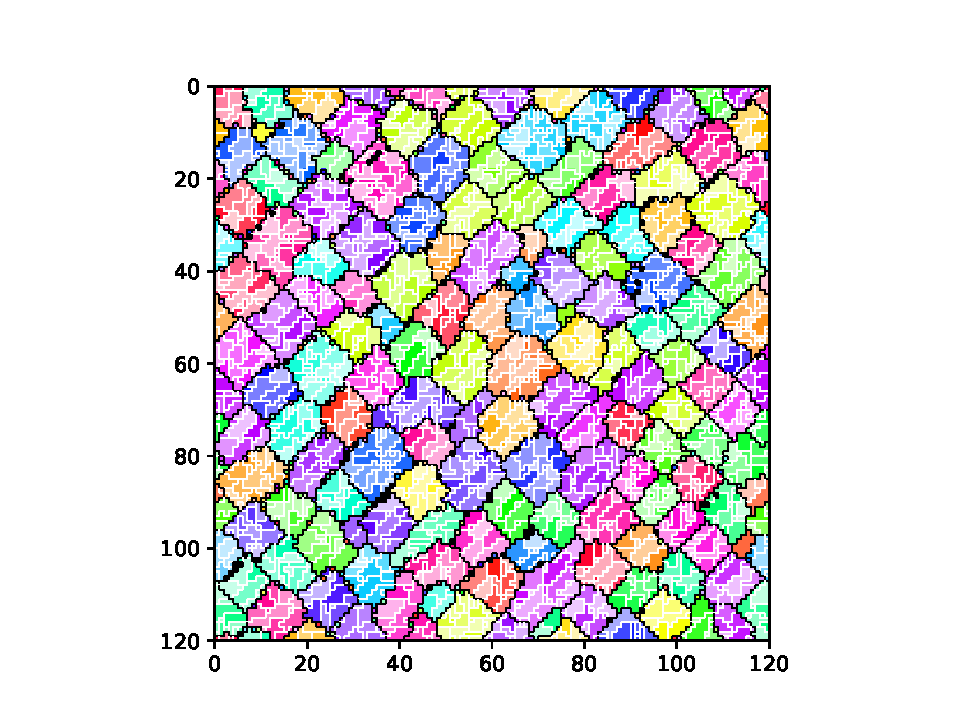
\includegraphics[width=\columnwidth,trim={2.5cm 0.5cm 2.5cm 1cm},clip]{img/ChannelMap_1022_update19500000}
  \caption{Mean $P_{c} = 0.77$, $P_0 = 0.089$, $P_1 = 0.14$; generation 20,475}
  \label{fig:ChannelMap_1022}
\end{subfigure}

\begin{subfigure}[b]{0.82\columnwidth}
  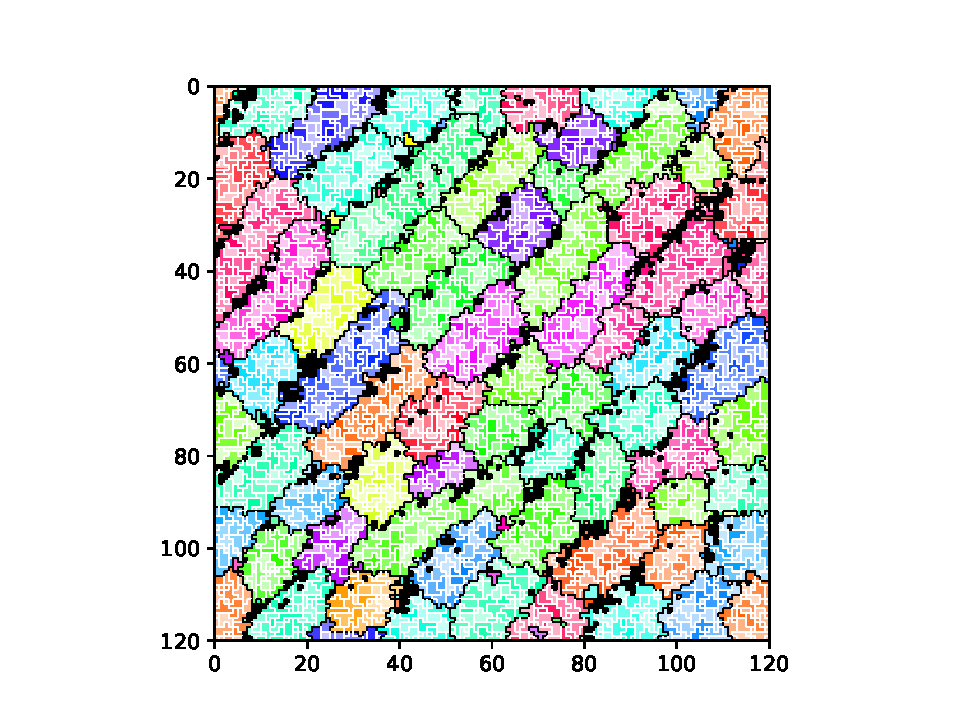
\includegraphics[width=\columnwidth,trim={2.5cm 0.5cm 2.5cm 1cm},clip]{img/ChannelMap_1041_update19500000}
  \caption{Mean $P_0 = 1.0$; generation 23,971}
  \label{fig:ChannelMap_1041}
\end{subfigure}

\begin{subfigure}[b]{0.82\columnwidth}
  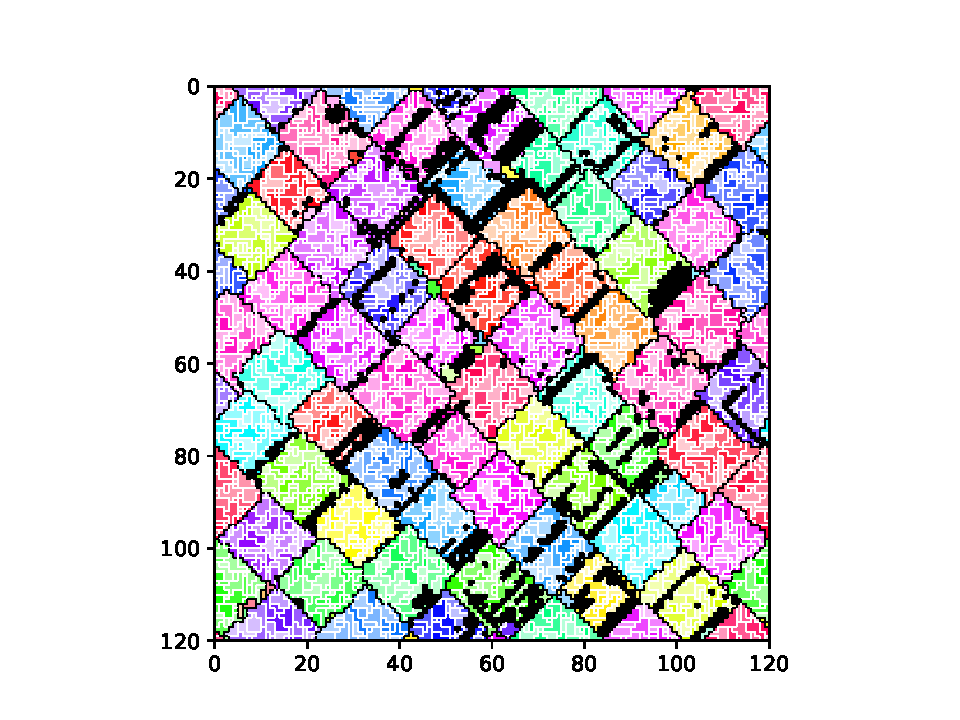
\includegraphics[width=\columnwidth,trim={2.5cm 0.5cm 2.5cm 1cm},clip]{img/ChannelMap_1008_update19500000}
  \caption{Mean $P_1 = 1.0$; generation 25,841}
  \label{fig:ChannelMap_1008}
\end{subfigure}

\caption{
State of same-channel level-zero and level-one signaling networks at the end of evolution with different population mean $P_{c}$, $P_0$, and $P_1$.
Level-zero channels coded by HSV value are separated by white borders and level-one channels coded by HSV hue are separated by black borders.
}
\label{fig:outcome_grids}
\end{center}
\end{figure}
